\documentclass{beamer}

\usetheme{Warsaw}
%\usetheme{CambridgeUS}

% modification history
% created on 18 sep 2011
% modified on 25 mar

%\usepackage{amsfonts, amsmath, amssymb}

%\setbeamertemplate{theorems}[numbered]
%\setbeamertemplate{theorems}[ams style] 
\usepackage[skins,breakable]{tcolorbox}
%\usepackage[normalem]{ulem}

%\usefonttheme[onlymath]{serif}                     // change the style of math font 

%=============set slide number=================
\addtobeamertemplate{navigation symbols}{}{
    \usebeamerfont{footline}
    \usebeamercolor[fg]{footline}
    \hspace{1em}
    \insertframenumber/\inserttotalframenumber
}
\setbeamercolor{footline}{fg=black}
\setbeamerfont{footline}{series=\bfseries}


%=============set footline=====================
\setbeamertemplate{footline}
{
  \leavevmode%
  \hbox{%
  \begin{beamercolorbox}[wd=.55\paperwidth,ht=2.25ex,dp=1ex,center]{author in head/foot}%
    \usebeamerfont{author in head/foot}\insertshortauthor
  \end{beamercolorbox}%
  \begin{beamercolorbox}[wd=.45\paperwidth,ht=2.25ex,dp=1ex,center]{title in head/foot}%
    \usebeamerfont{title in head/foot}\insertshorttitle
  \end{beamercolorbox}}%
  \vskip0pt%
}

%creating a rectangle box def
\newtcbox{\mybox}[1][red]{arc=0pt,outer arc=0pt,colback=#1!10!white,colframe=#1!50!black, boxsep=0pt,left=1pt,right=1pt,top=2pt,bottom=2pt,boxrule=0pt,bottomrule=1pt,toprule=1pt}

\newtcbox{\xmybox}[1][red]{arc=7pt,colback=#1!10!white,colframe=#1!50!black,before upper={\rule[-3pt]{0pt}{10pt}},boxrule=1pt,boxsep=0pt,left=6pt,right=6pt,top=2pt,bottom=2pt}
%the ``on line'' option doesn't work. so omitting it

%===== spacing =====

\def\extraspacing{\vspace{2mm} \noindent}
\def\vgap{\vspace{2mm}}
\def\hgap{\textrm{\hspace{1mm}}}

%===== tabbing =====

\def\tab{\hspace{2mm}}
\def\tabpos{\hspace{4mm} \= \hspace{4mm} \= \hspace{4mm} \= \hspace{4mm} \=
\hspace{4mm} \= \hspace{4mm} \= \hspace{4mm} \= \hspace{4mm} \= \hspace{4mm}
\kill}
\newcommand{\mytab}[1]{\begin{tabbing}\tabpos #1\end{tabbing}}

%===== blocks =====

% \newtheorem{theorem}{Theorem}
% \newtheorem{lemma}{Lemma}
% \newtheorem{corollary}{Corollary}
% \newtheorem{proposition}{Proposition}
% \newtheorem{definition}{Definition}
% \newtheorem{problem}{Problem}

\newcommand{\cbox}[2]{\begin{tcolorbox}[arc=0mm, colframe=#1!50!black, colback=#1!10!white]#2\end{tcolorbox}}
\newcommand{\minipg}[2]{\begin{center}\begin{minipage}{#1}#2\end{minipage}\end{center}}
\newcommand{\myfrm}[1]{\begin{frame}\begin{small}#1\end{small}\end{frame}} 
\newcommand{\myitems}[1]{\begin{itemize}#1\end{itemize}}
\newcommand{\myenums}[1]{\begin{enumerate}#1\end{enumerate}}
\newcommand{\myfig}[1]{\begin{figure}\centering #1\end{figure}}
    
%===== math macros =====
\newcommand{\bm}[1]{\textrm{\boldmath${#1}$}}
%\newcommand{\smat}[2]{\left[\begin{tabular}{#1}#2\end{tabular}\right]}
%\newcommand{\bmat}[2]{\left|\begin{tabular}{#1}#2\end{tabular}\right|}
\newcommand{\bmat}[1]{\begin{bmatrix}#1\end{bmatrix}}
\newcommand{\vmat}[1]{\begin{vmatrix}#1\end{vmatrix}}
\newcommand{\myeqn}[1]{\begin{eqnarray}#1\end{eqnarray}}
\newcommand{\set}[1]{\{#1\}}

\def\eps{\epsilon}
\def\fr{\frac}
\def\lc{\lceil}
\def\lf{\lfloor}
\def\rc{\rceil}
\def\rf{\rfloor}
\def\Pr{\textrm{\boldmath$Pr$}}
\def\expt{\textrm{\boldmath$E$}}
\def\real{\mathbb{R}}
\def\int{\mathbb{Z}}
\def\*{\star}
\def\tO{\tilde{O}}

\DeclareMathOperator*{\argmin}{arg\,min}
\DeclareMathOperator*{\polylg}{polylg}
\DeclareMathOperator*{\polylog}{polylog}
\DeclareMathOperator*{\intr}{\cap}

\def\nn{\nonumber}
\def\mit{\mathit}


%===== misc =====

\def\done{\hspace*{\fill} $\framebox[2mm]{}$}	% end of proof
\def\ttt{\texttt}

%===== coloring =====
\newcommand{\red}[1]{\textcolor{red}{#1}}
\newcommand{\bred}[1]{\textcolor{red}{\bf #1}}
\newcommand{\blue}[1]{\textcolor{blue}{\bf #1}}

\usepackage{color}
\usepackage{graphicx}
\usepackage{multirow}
\usepackage{wrapfig}
\usepackage[skins,breakable]{tcolorbox}

\def\done{\hfill$\square$}
\def\ttt{\texttt}
\def\vgap{\vspace{5mm}}

\def\sort{\mit{sort}}

\title[DATABASE SYSTEM PRINCIPLES]{Query Processing 5:\\ Query Optimization}

\author[Yufei Tao @ NTU]{Yufei Tao}
\institute[]{\url{https://www.cse.cuhk.edu.hk/~taoyf}}
\date{}

% \def\dtm{\mathit{d\mbox{-}tm}}
% \def\ftm{\mathit{f\mbox{-}tm}}
\def\bestext{\mathit{best\mbox{-}ext}}

\begin{document}
%-------------------------------------------------------------
\begin{frame}
    \titlepage
%     \begin{tcolorbox}[arc=0mm, colframe=green!50!black, colback=green!10!white] 
%     \end{tcolorbox}
\end{frame}
%-------------------------------------------------------------
\begin{frame}
\begin{small}
    This lecture will provide an overview of \bred{query optimization}, which is a process carried out by a database to select a query execution strategy.
    %\vgap
\end{small}    
\end{frame}
%-------------------------------------------------------------
\myfrm{
    \xmybox{Example}

    \vgap

    Relations $\red{R_1(A, B)}$ and $\red{R_2(B, C)}$. \\
    SQL query:
    \mytab{
        \> \ttt{SELECT} $A, C$ \ttt{FROM} $R, S$ \\
        \> \ttt{WHERE} $R_1.B = R_2.B$ \ttt{AND} $S.B = 1$ \ttt{AND} $S.C$ \ttt{BETWEEN} 100 \ttt{AND} 200
    }

    \cbox{green}{
    A query plan:
    \begin{center}
        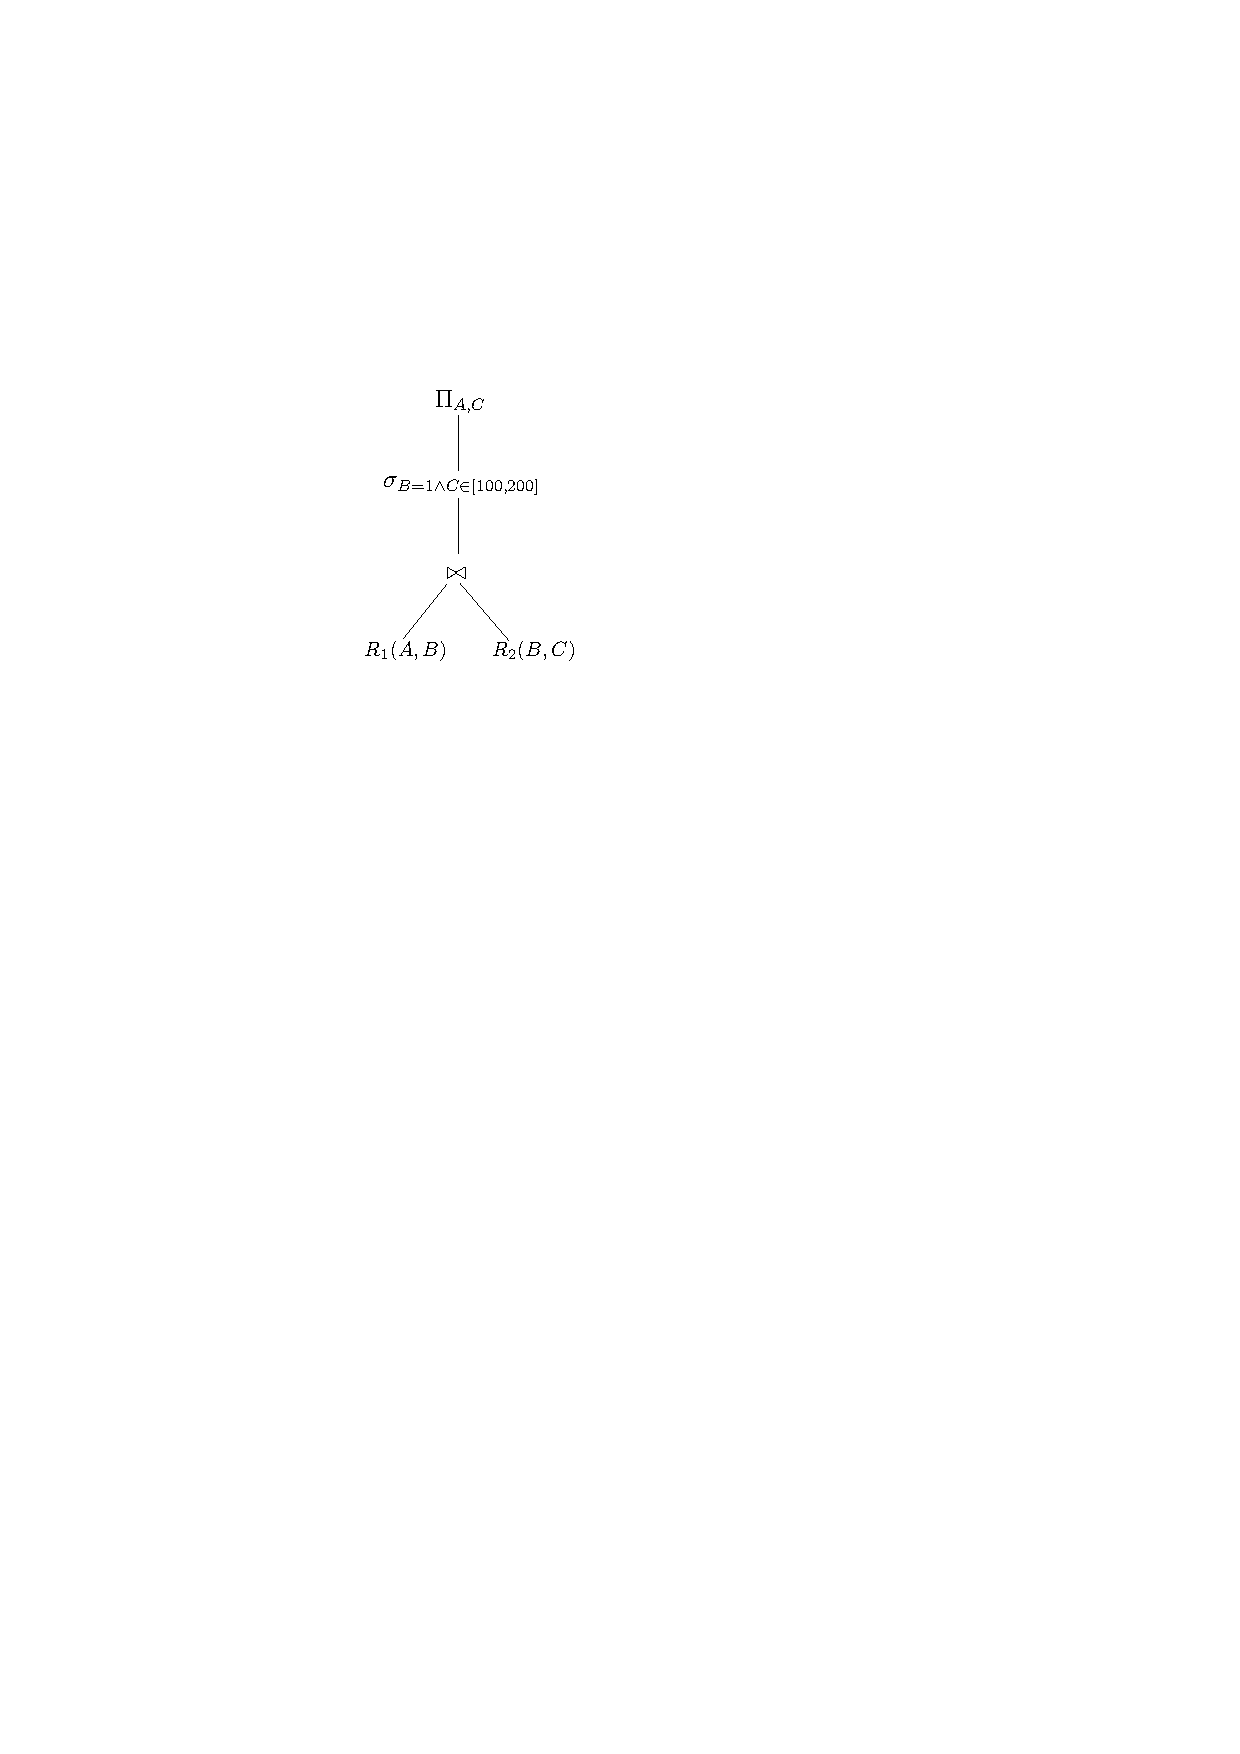
\includegraphics[height=30mm]{./artwork/plan1}
    \end{center}
    }
}
%-------------------------------------------------------------
\myfrm{
    \cbox{blue}{
        Before running a query plan, the database always estimates its cost.
    }
}
%-------------------------------------------------------------
\myfrm{

    \begin{tabular}{cc}
        %\minipg{0.5\linewidth}{
        \begin{minipage}{0.7\linewidth}
            Assume:
            \myitems{
                \item $\red{B(R_1)} = \red{B(R_2)} = 10000$ \\
                (i.e., each relation has 10000 blocks). \\[-1mm]
                \item $R_1 \bowtie R_2$ has $\red{B_1}$ blocks. \\[-1mm]
                \item $\sigma_{B = 1 \wedge C \in [100,200]} R_1 \bowtie R_2$ has $\red{B_2}$ blocks. \\[-1mm]
                \item $\red{M} = 101$ (the memory has 101 blocks).
            }
        \end{minipage}
        &
        \begin{minipage}{0.2\linewidth}
            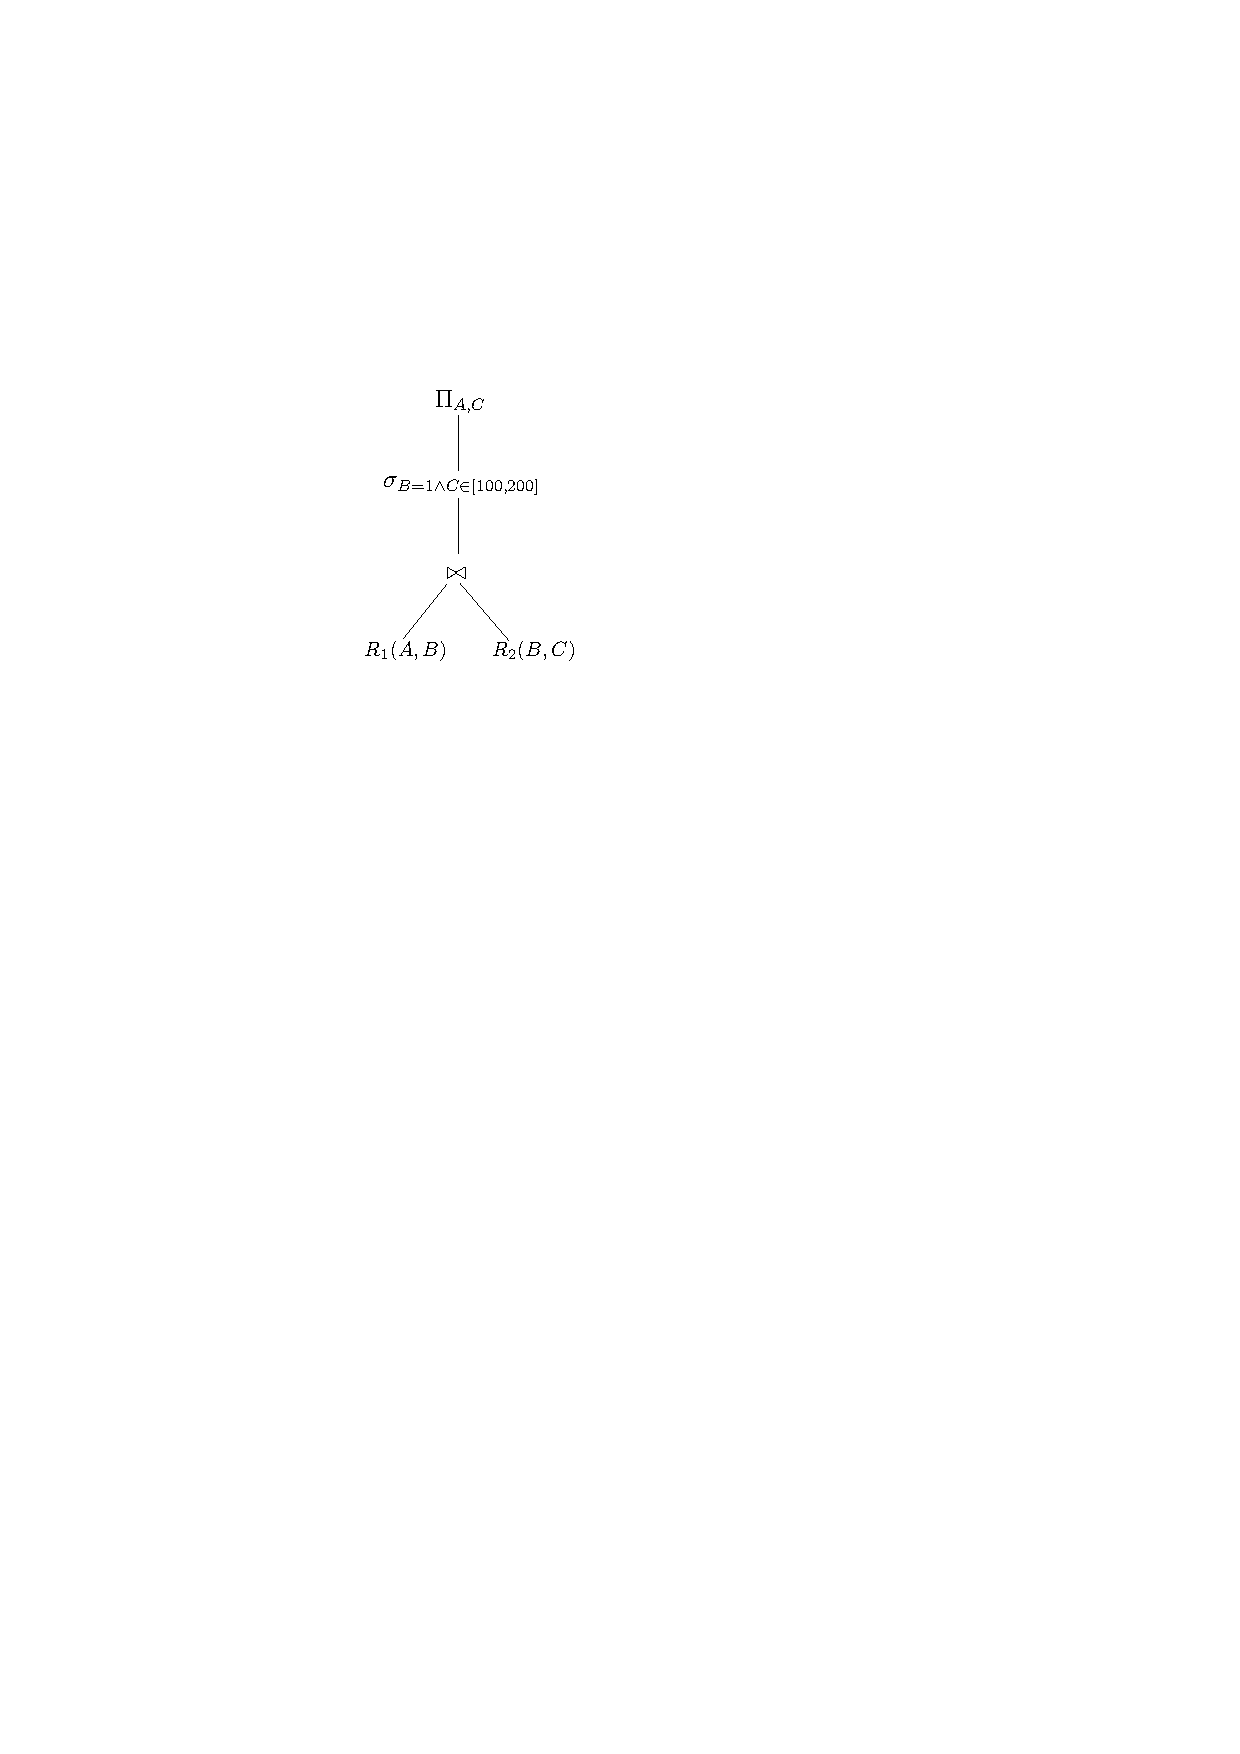
\includegraphics[height=30mm]{./artwork/plan1}
        \end{minipage}
    \end{tabular}

    \vgap

    \mybox[green]{Strategy 1:}
    \begin{itemize}
        \item Compute $\red{R_3} = R_1 \bowtie R_2$ with BNL and \blue{materialize} $R_3$ (i.e., write $R_3$ to the disk)
                $\Rightarrow$ $10^4 + 10^6$ I/Os (BNL) + $B_1$ (mat.).
        \item Compute $\red{R_4} = \sigma_{B = 1 \wedge C \in [100,200](R_3)}$ by reading $R_3$ and materializing $R_4$
                $\Rightarrow$ $B_1$ (reading) + $B_2$ (materialization) I/Os.
        \item Compute $\Pi_{A,C}(R_4)$ by reading $R_4$ $\Rightarrow$ $B_2$ I/Os.
    \end{itemize}
    In total: $1010000 + 2(B_1 + B_2)$ I/Os.
}
%-------------------------------------------------------------
\myfrm{
    Next, we will see several generic methods for improving the strategy.

    \vgap

    \cbox{yellow}{
        \centering
        \blue{Method 1:} Algorithm Selection
    }
}
%-------------------------------------------------------------
\myfrm{

    \begin{tabular}{cc}
        %\minipg{0.5\linewidth}{
        \begin{minipage}{0.7\linewidth}
            Assume:
            \myitems{
                \item $\red{B(R_1)} = \red{B(R_2)} = 10000$ \\[-1mm]
                \item $R_1 \bowtie R_2$ has $\red{B_1}$ blocks. \\[-1mm]
                \item $\sigma_{B = 1 \wedge C \in [100,200]} R_1 \bowtie R_2$ has $\red{B_2}$ blocks. \\[-1mm]
                \item $\red{M} = 101$.
            }
        \end{minipage}
        &
        \begin{minipage}{0.2\linewidth}
            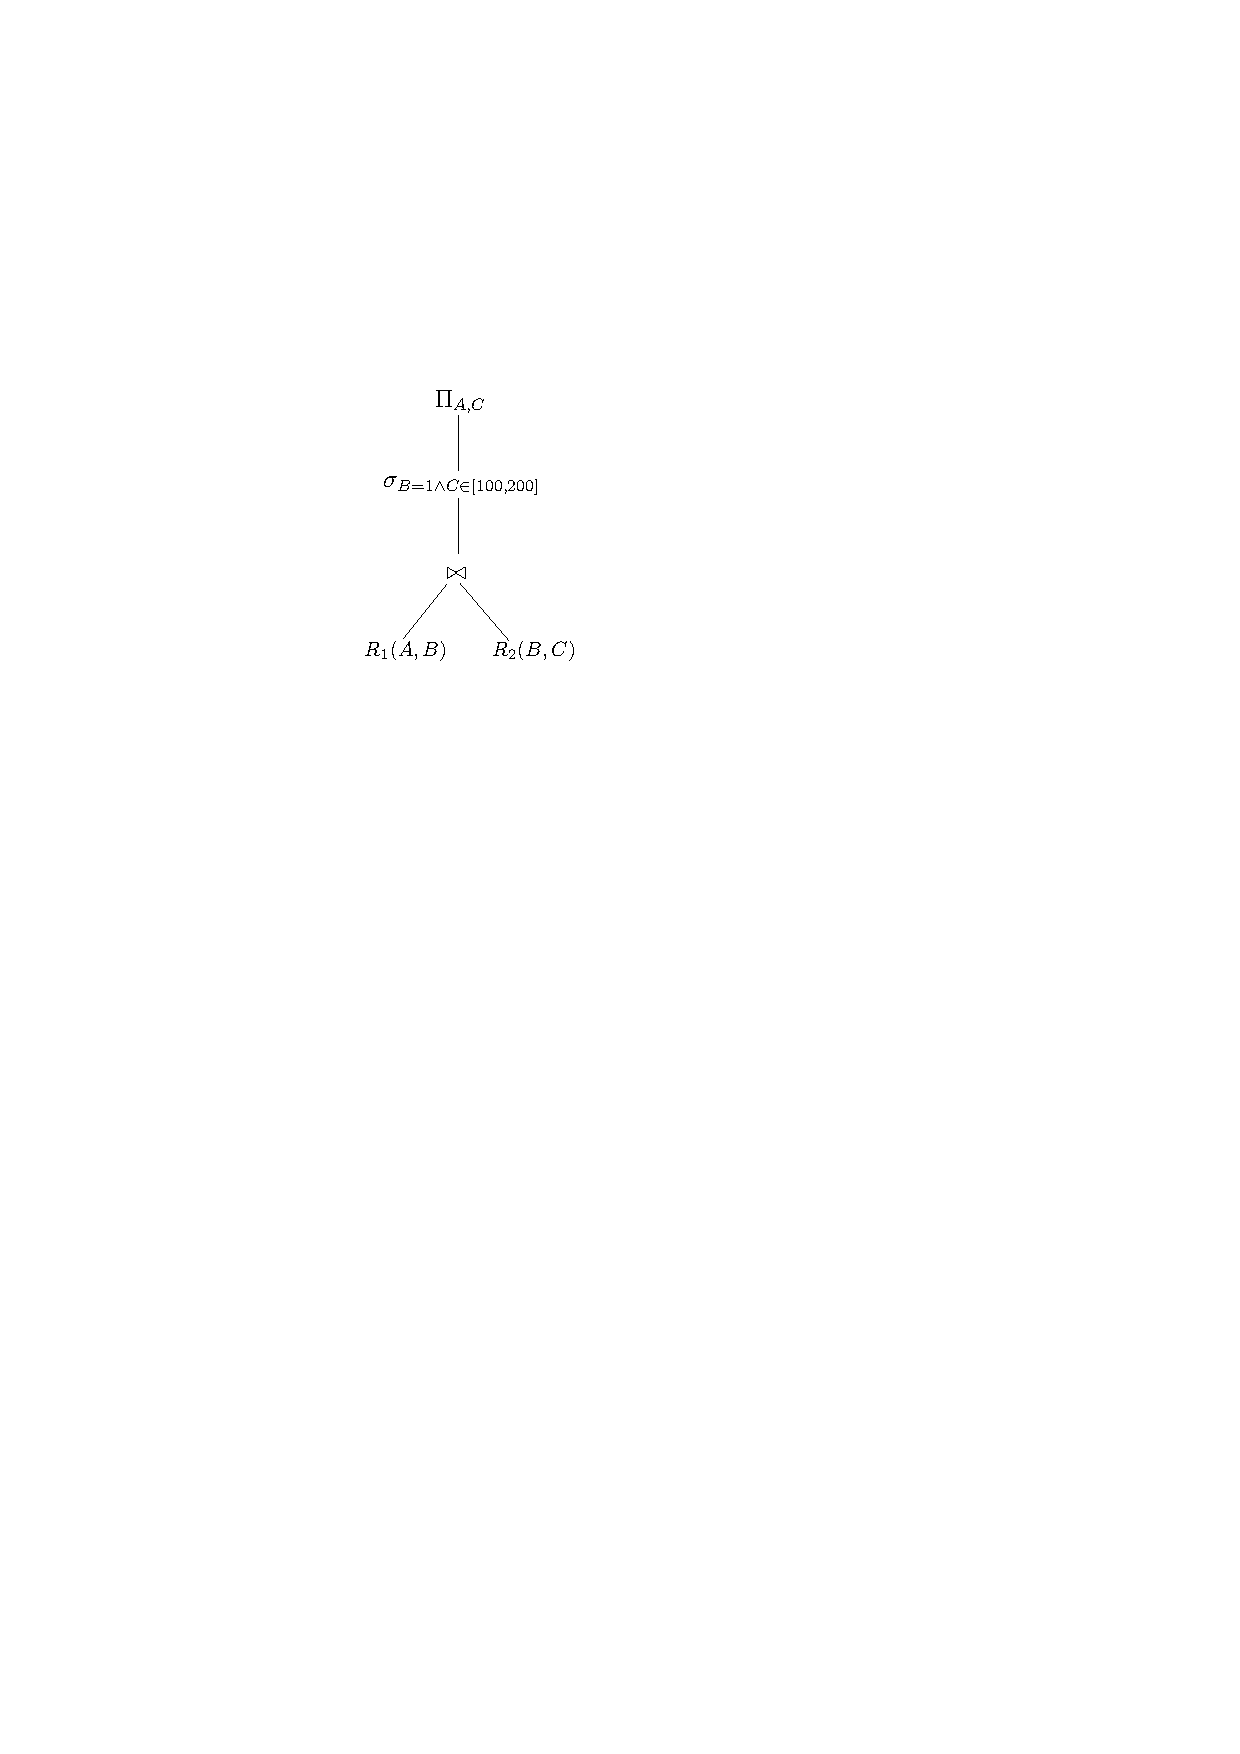
\includegraphics[height=30mm]{./artwork/plan1}
        \end{minipage}
    \end{tabular}

    \vgap

    \mybox[green]{Strategy 2:}
    \begin{itemize}
        \item Compute $\red{R_3} = R_1 \bowtie R_2$ with \bred{sort join} and materialize $R_3$
                $\Rightarrow$ $5(10^4 + 10^4)$ I/Os (\bred{under no-skew assumption}) + $B_1$ (mat.).
        \item Compute $\red{R_4} = \sigma_{B = 1 \wedge C \in [100,200](R_3)}$ by reading $R_3$ and materializing $R_4$
                $\Rightarrow$ $B_1$ (reading) + $B_2$ (materialization) I/Os.
        \item Compute $\Pi_{A,C}(R_4)$ by reading $R_4$ $\Rightarrow$ $B_2$ I/Os.
    \end{itemize}
    In total: $100000 + 2(B_1 + B_2)$ I/Os.
}
%-------------------------------------------------------------
\myfrm{
    \cbox{yellow}{
        \centering
        \blue{Method 2:} Query Rewriting
    }
}
%-------------------------------------------------------------
\myfrm{
    Observe:
    \myeqn{
        && \Pi_{A,C}(\sigma_{B=1 \wedge C \in [100, 200]} (R_1 \bowtie R_2) \nn \\
        &=&
        \Pi_{A,C}(\sigma_{B=1}(R_1) \bowtie \sigma_{B=1 \wedge C \in [100, 200]} (R_2)) \nn
    }

    %\vgap

    \cbox{blue}{
        \blue{Query rewriting} converts the original query to an equivalent query using laws of relational algebra.
    }

    \begin{center}
        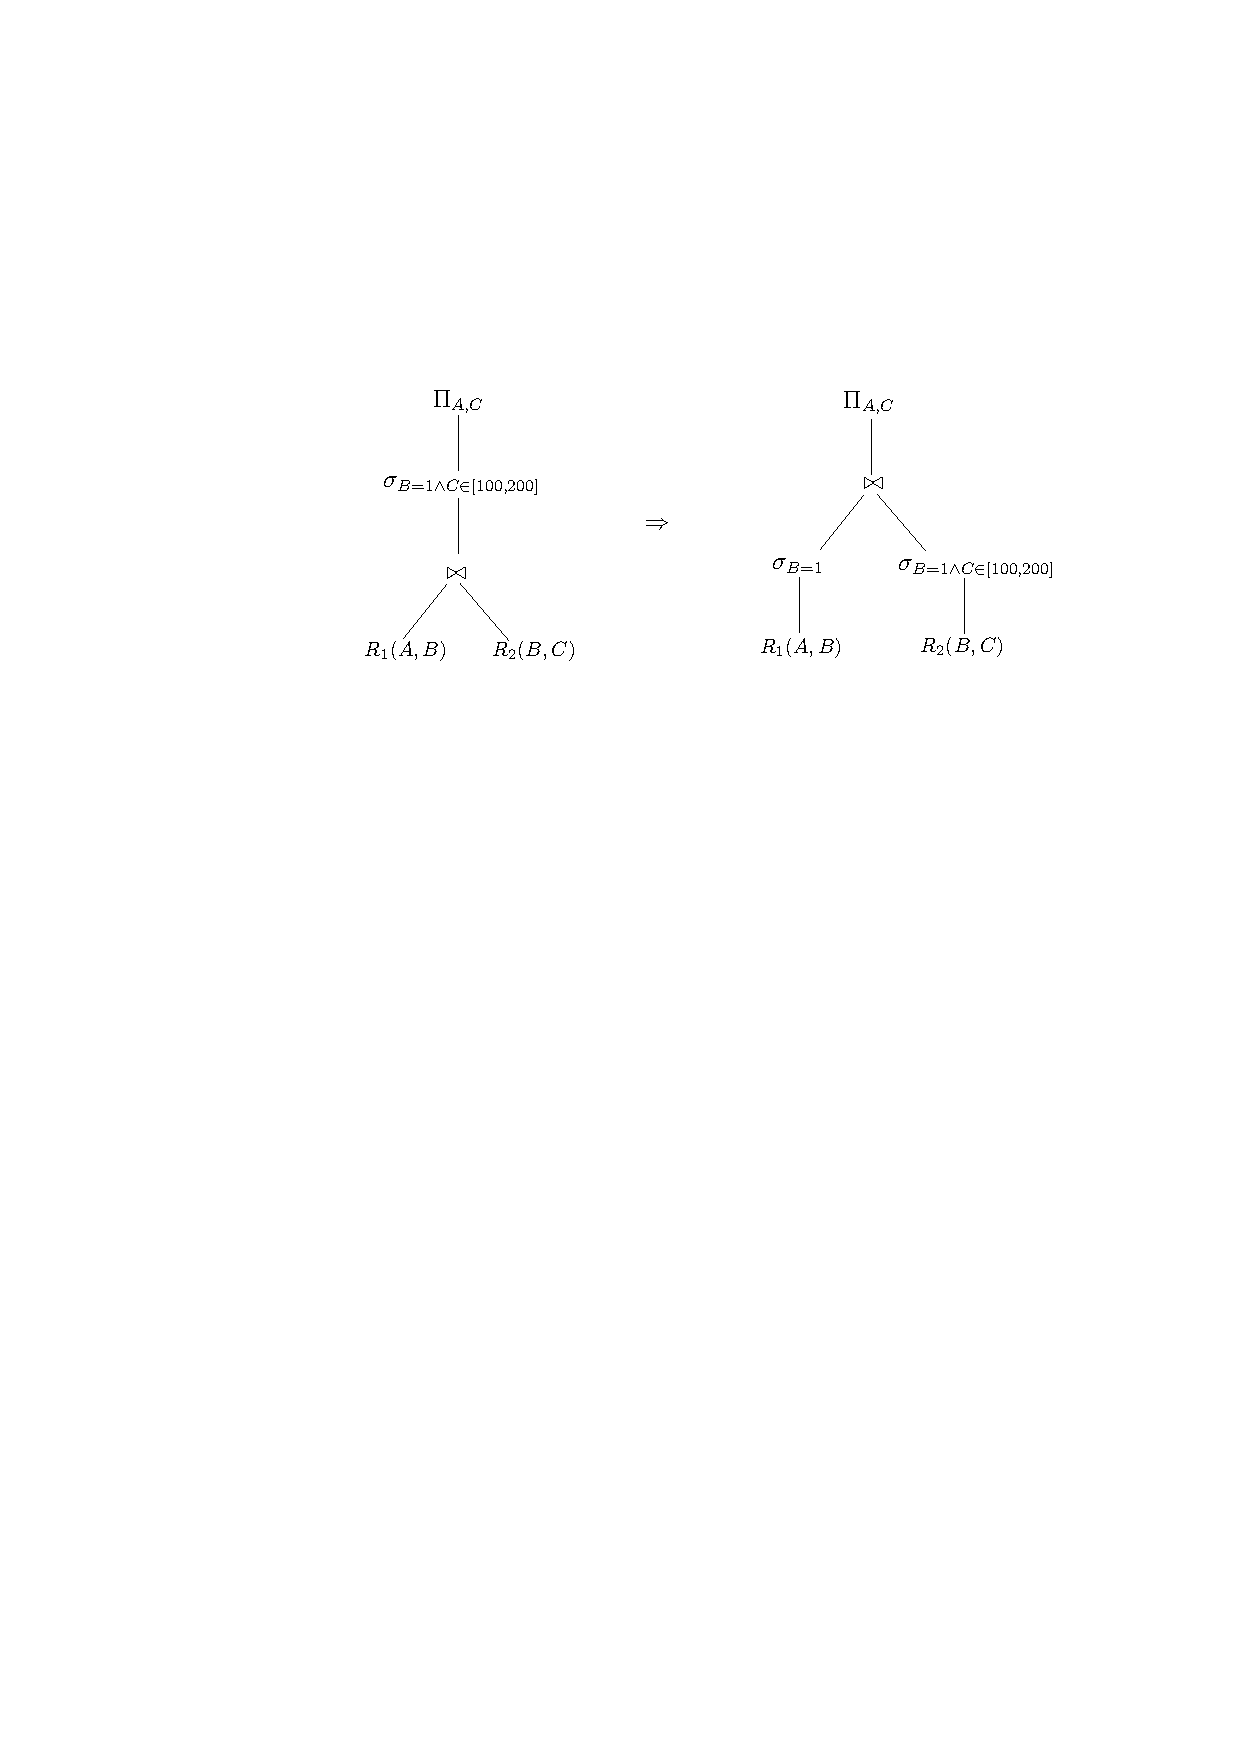
\includegraphics[height=30mm]{./artwork/plan1.5}
    \end{center}

    \cbox{green}{
        \bred{Rule of thumb:} In practice, selections are almost always pushed down as much as possible.
    }
}
%-------------------------------------------------------------
\myfrm{

    \begin{tabular}{cc}
        %\minipg{0.5\linewidth}{
        \begin{minipage}{0.7\linewidth}
            Assume:
            \myitems{
                \item $\red{B(R_1)} = \red{B(R_2)} = 10000$ \\[-1mm]
                %\item $R_1 \bowtie R_2$ has $\red{B_1}$ blocks. \\[-1mm]
                \item $\sigma_{B = 1} R_1 $ has $1000$ blocks  \\[-1mm]
                \item $\sigma_{B = 1 \wedge C \in [100, 200]} R_2$ has $800$ blocks  \\[-1mm]
                \item $\sigma_{B = 1 \wedge C \in [100,200]} R_1 \bowtie R_2$ has $\red{B_2}$ blocks. \\[-1mm]
                \item $\red{M} = 101$.
            }
        \end{minipage}
        &
        \begin{minipage}{0.2\linewidth}
            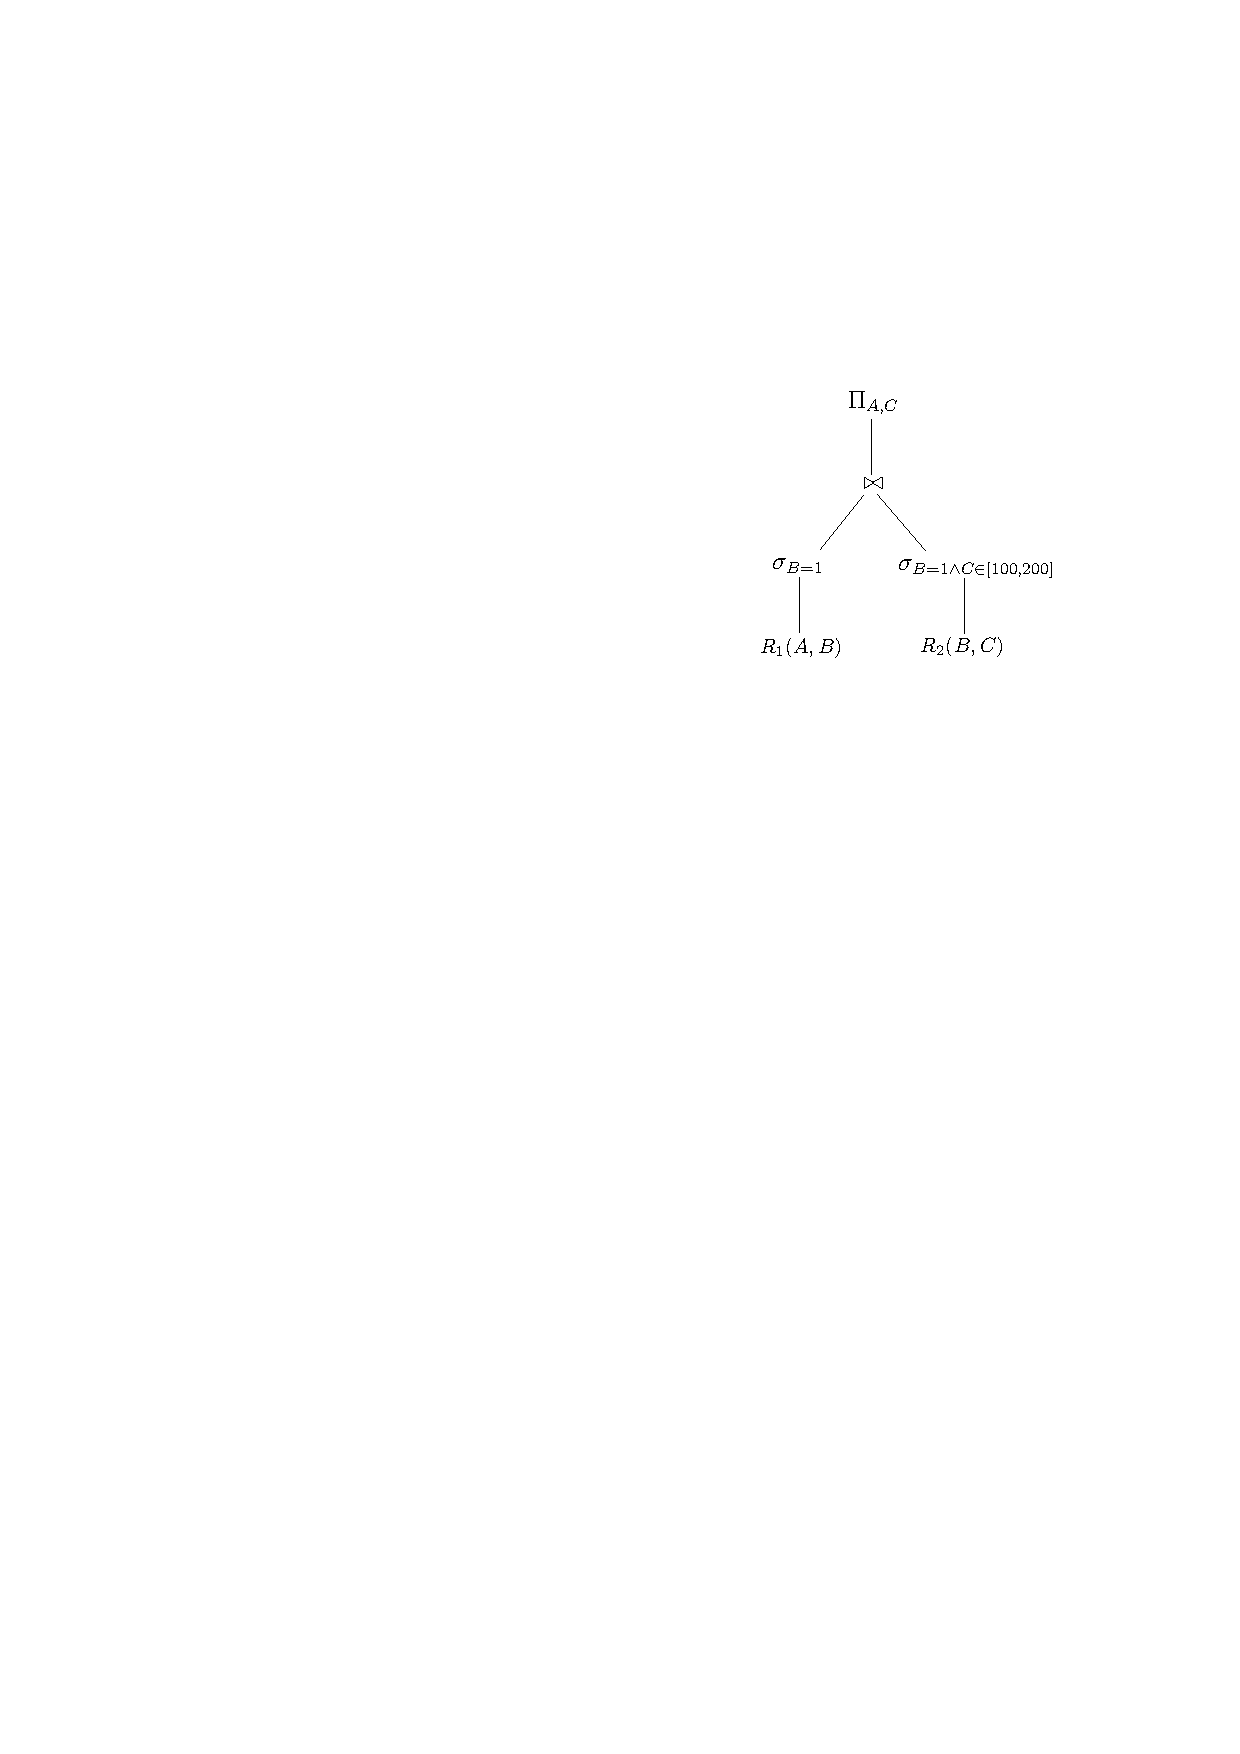
\includegraphics[height=30mm]{./artwork/plan2}
        \end{minipage}
    \end{tabular}

    \vgap

    \mybox[green]{Strategy 3:}
    \begin{itemize}
        \item Compute $\red{R_3} = \sigma_{B=1} R_1$ by reading $R_1$ and materializing $R_3$ \\
        $\Rightarrow$ 10000 (reading) + 1000 (mat.) I/Os \\[-1mm]
        \item Compute $\red{R_4} = \sigma_{B=1 \wedge C \in [100, 200]} R_2$ by reading $R_2$ and materializing $R_4$ $\Rightarrow$ 10000 (reading) + 800 (mat.) I/Os \\[-1mm]
        \item Compute $\red{R_5} = R_3 \bowtie R_4$ with sort join and materialize $R_5$
                $\Rightarrow$ $5(1000 + 800)$ I/Os (under no-skew assumption) + $B_2$ (mat.). \\[-1mm]
        \item Compute $\Pi_{A,C}(R_5)$ by reading $R_5$ $\Rightarrow$ $B_2$ I/Os.
    \end{itemize}
    In total: $30800 + 2 B_2$ I/Os.
}
%-------------------------------------------------------------
\myfrm{
    \cbox{yellow}{
        \centering
        \blue{Method 3:} Applying Indexes
    }
}
%-------------------------------------------------------------
\myfrm{
    \begin{tabular}{cc}
        %\minipg{0.5\linewidth}{
        \hspace{-5mm}
        \begin{minipage}{0.75\linewidth}
            Assume:
            \myitems{
                \item $\red{B(R_1)} = \red{B(R_2)} = 10000$ \\[-1mm]
                \item $\sigma_{B = 1} R_1 $ has $1000$ blocks  \\[-1mm]
                \item $\sigma_{C \in [100, 200]} R_2$ has 3000 blocks \\[-1mm]
                \item $R_2$ is \bred{clustered} on $C$. \\
                There is a \bred{B-tree} on $R_2.C$ with 3 levels. \\ [-1mm]
                \item $\sigma_{B = 1 \wedge C \in [100, 200]} R_2$ has $800$ blocks  \\[-1mm]
                \item $\sigma_{B = 1 \wedge C \in [100,200]} R_1 \bowtie R_2$ has $\red{B_2}$ blocks. \\[-1mm]
                \item $\red{M} = 101$.
            }
        \end{minipage}
        &
        \begin{minipage}{0.2\linewidth}
            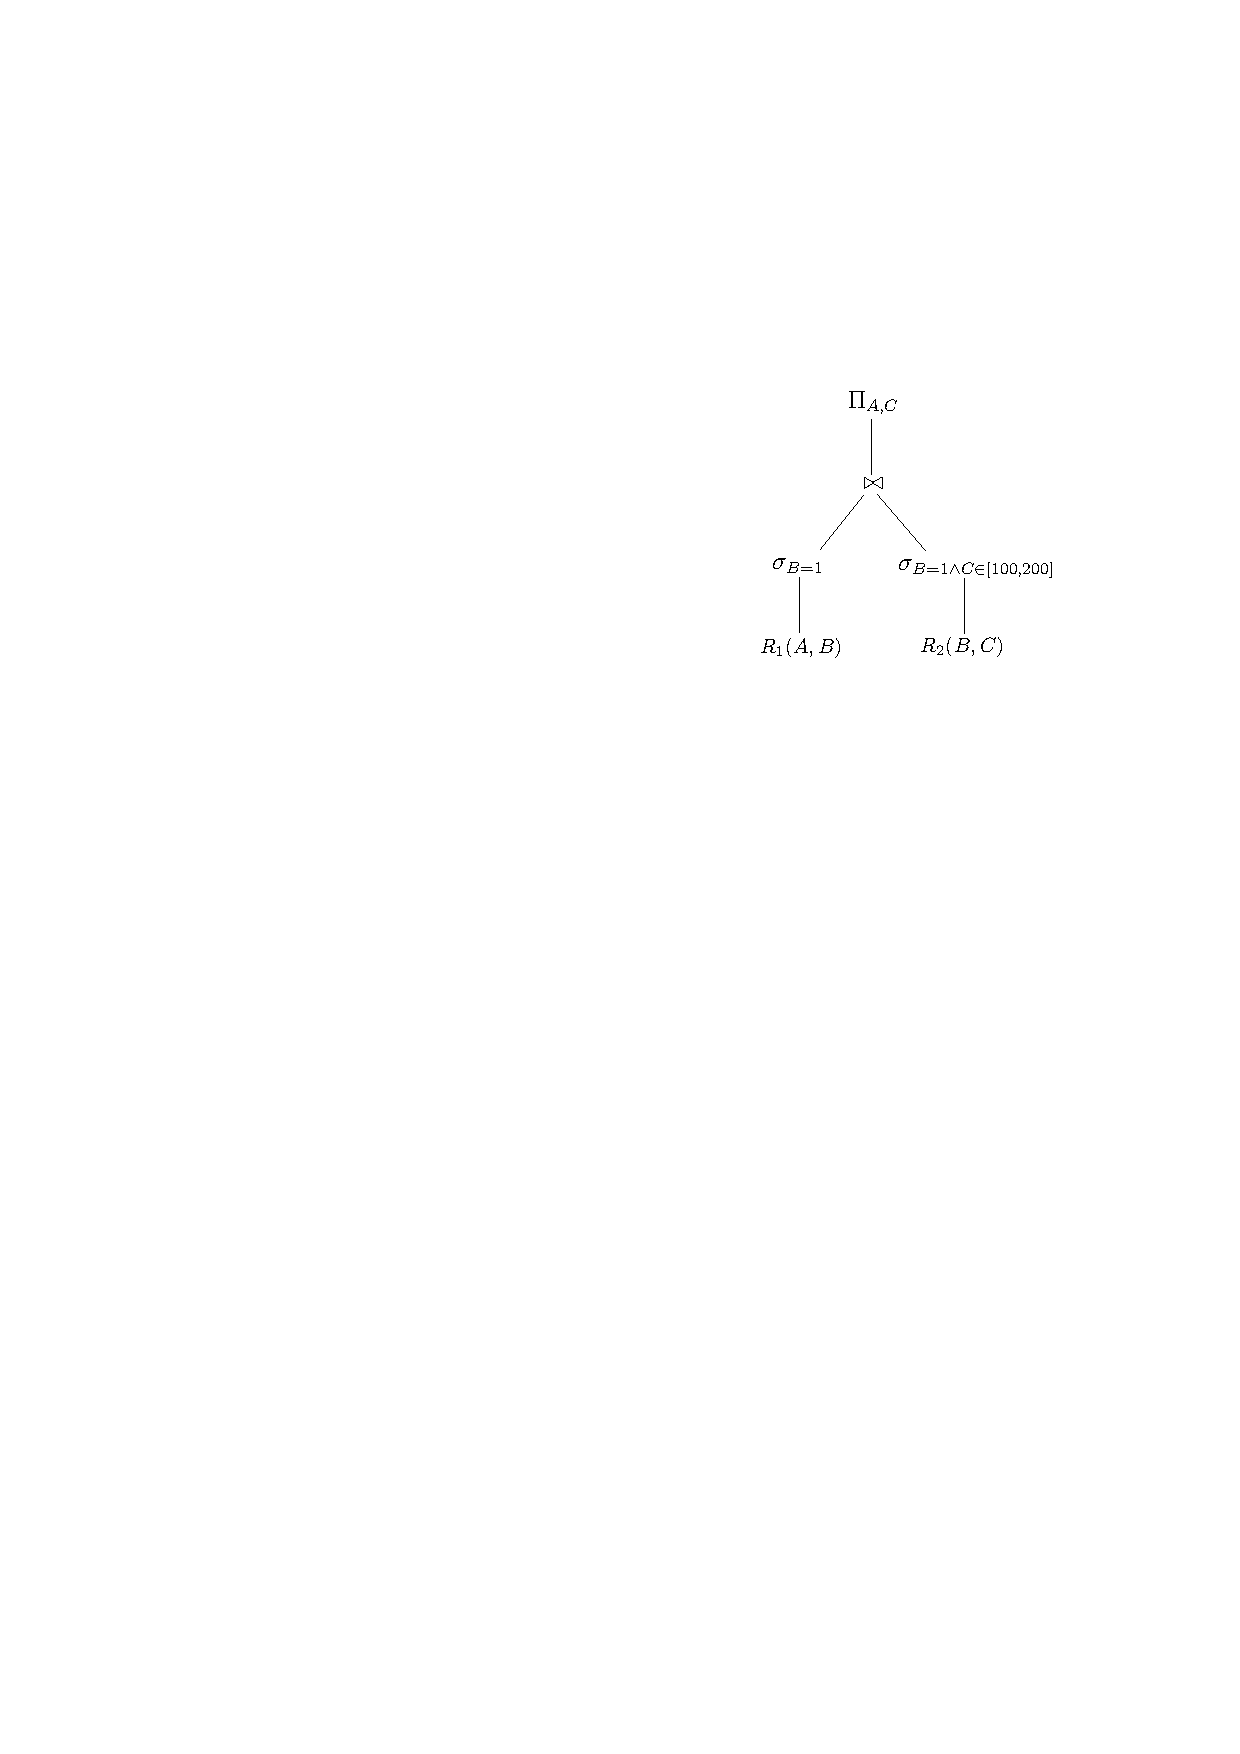
\includegraphics[height=30mm]{./artwork/plan2}
        \end{minipage}
    \end{tabular}

    \vgap


}
%-------------------------------------------------------------
\myfrm{
    \mybox[green]{Strategy 4:}
    \begin{center}
            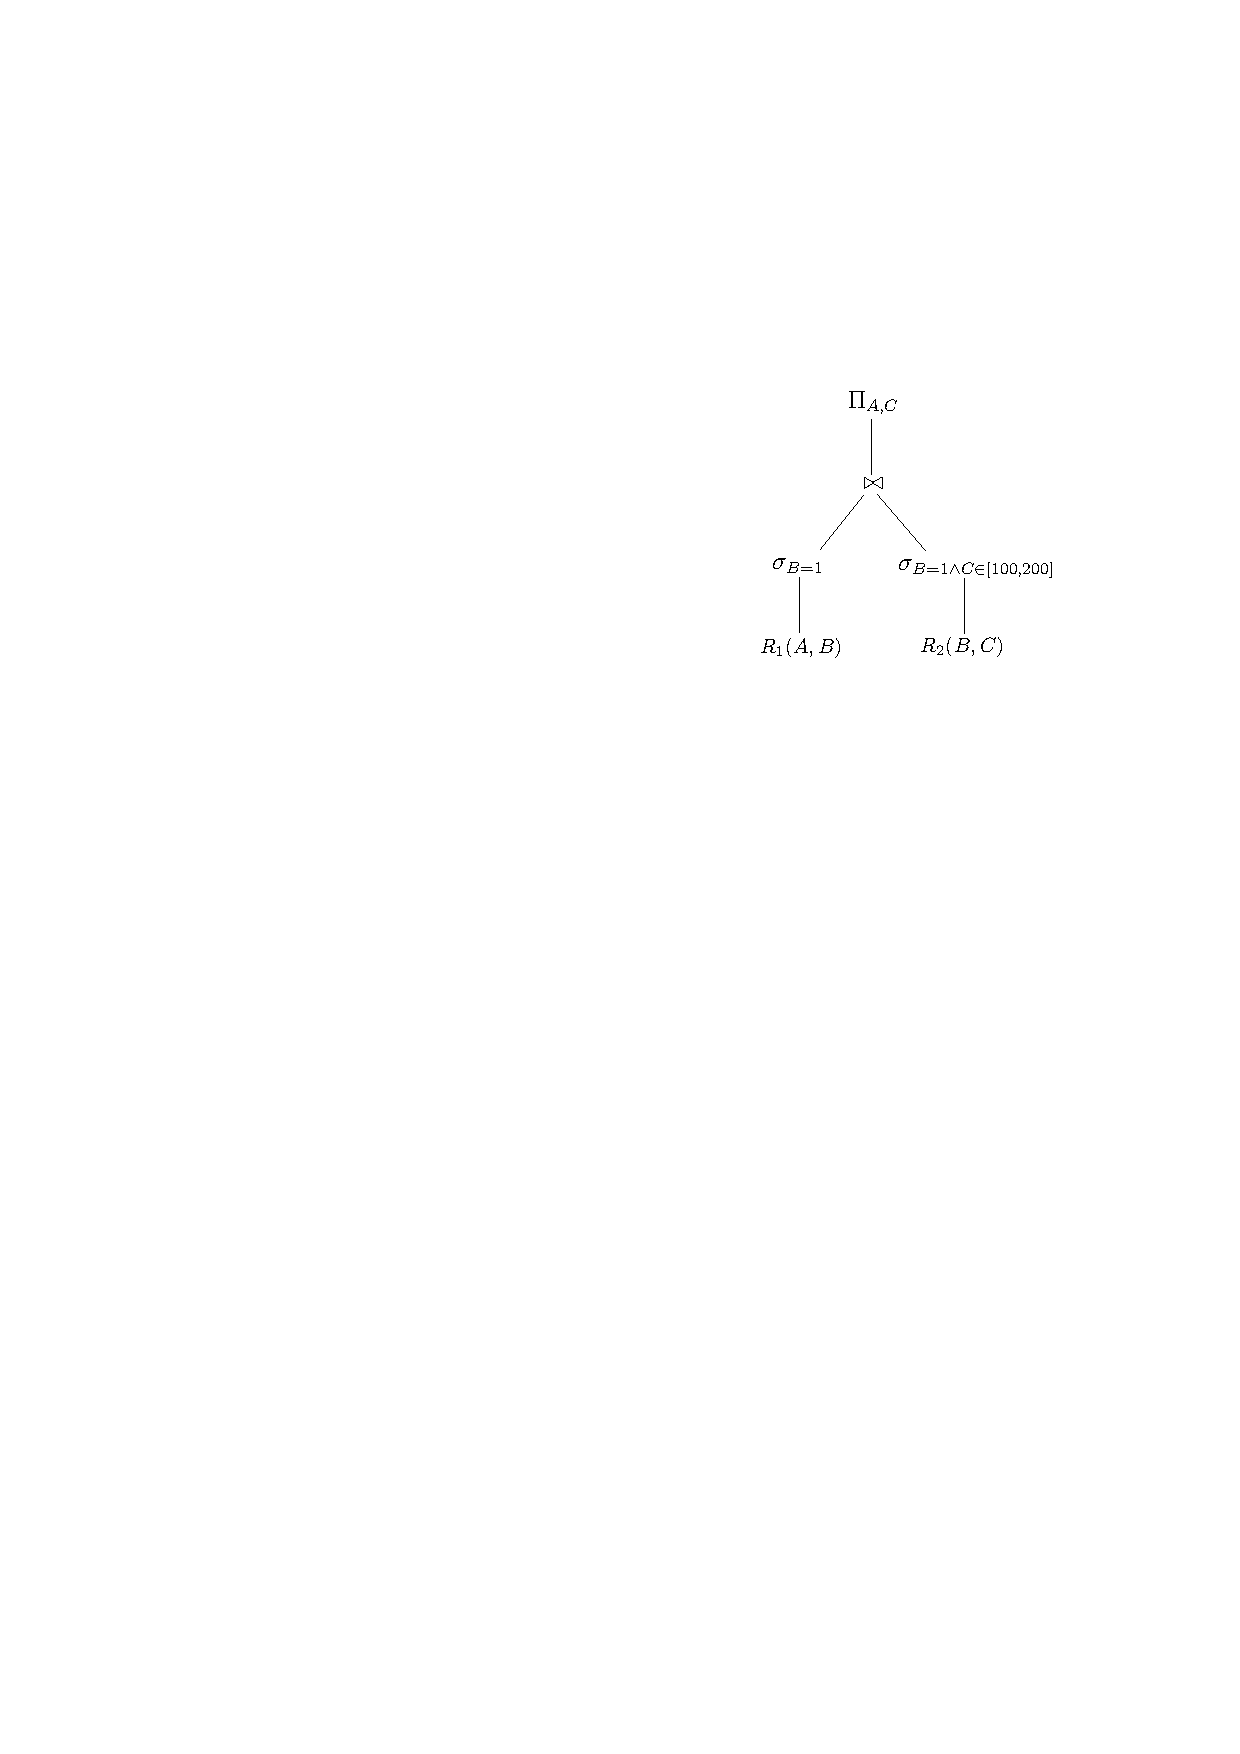
\includegraphics[height=30mm]{./artwork/plan2} \vspace{-5mm}
    \end{center}

    \begin{itemize}
        \item Compute $\red{R_3} = \sigma_{B=1} R_1$ by reading $R_1$ and materializing $R_3$ \\
        $\Rightarrow$ 10000 (reading) + 1000 (mat.) I/Os \\[-1mm]
        \item Compute $\red{R_4} = \sigma_{B=1 \wedge C \in [100, 200]} R_2$ by using the B-tree on $R_2.C$ and materialize $R_4$ $\Rightarrow$ 3 (B-tree) + 3000 (retrieving $\sigma_{C \in [100, 200]} R_2$) + 800 (mat.) I/Os \\[-1mm]
        \item Compute $\red{R_5} = R_3 \bowtie R_4$ with sort join and materialize $R_5$
                $\Rightarrow$ $5(1000 + 800)$ I/Os (under no-skew assumption) + $B_2$ (mat.). \\[-1mm]
        \item Compute $\Pi_{A,C}(R_5)$ by reading $R_5$ $\Rightarrow$ $B_2$ I/Os.
    \end{itemize}
    In total: $23803 + 2 B_2$ I/Os.
}
%-------------------------------------------------------------
\myfrm{
    \cbox{yellow}{
        \centering
        \blue{Method 4:} Pipelining
    }

    \vgap

    \cbox{blue}{
        \blue{Pipelining} processes multiple operations in a query plan \bred{together}.
    }
}
%-------------------------------------------------------------
\myfrm{
    \begin{tabular}{cc}
        %\minipg{0.5\linewidth}{
        \begin{minipage}{0.7\linewidth}
            Assume:
            \myitems{
                \item $\red{B(R_1)} = \red{B(R_2)} = 10000$ \\[-1mm]
                %\item $R_1 \bowtie R_2$ has $\red{B_1}$ blocks. \\[-1mm]
                \item $\sigma_{B = 1} R_1 $ has $1000$ blocks  \\[-1mm]
                \item $\sigma_{B = 1 \wedge C \in [100, 200]} R_2$ has $800$ blocks  \\[-1mm]
                %\item $\sigma_{B = 1 \wedge C \in [100,200]} R_1 \bowtie R_2$ has $\red{B_2}$ blocks. \\[-1mm]
                \item $\red{M} = 101$.
            }
        \end{minipage}
        &
        \begin{minipage}{0.2\linewidth}
            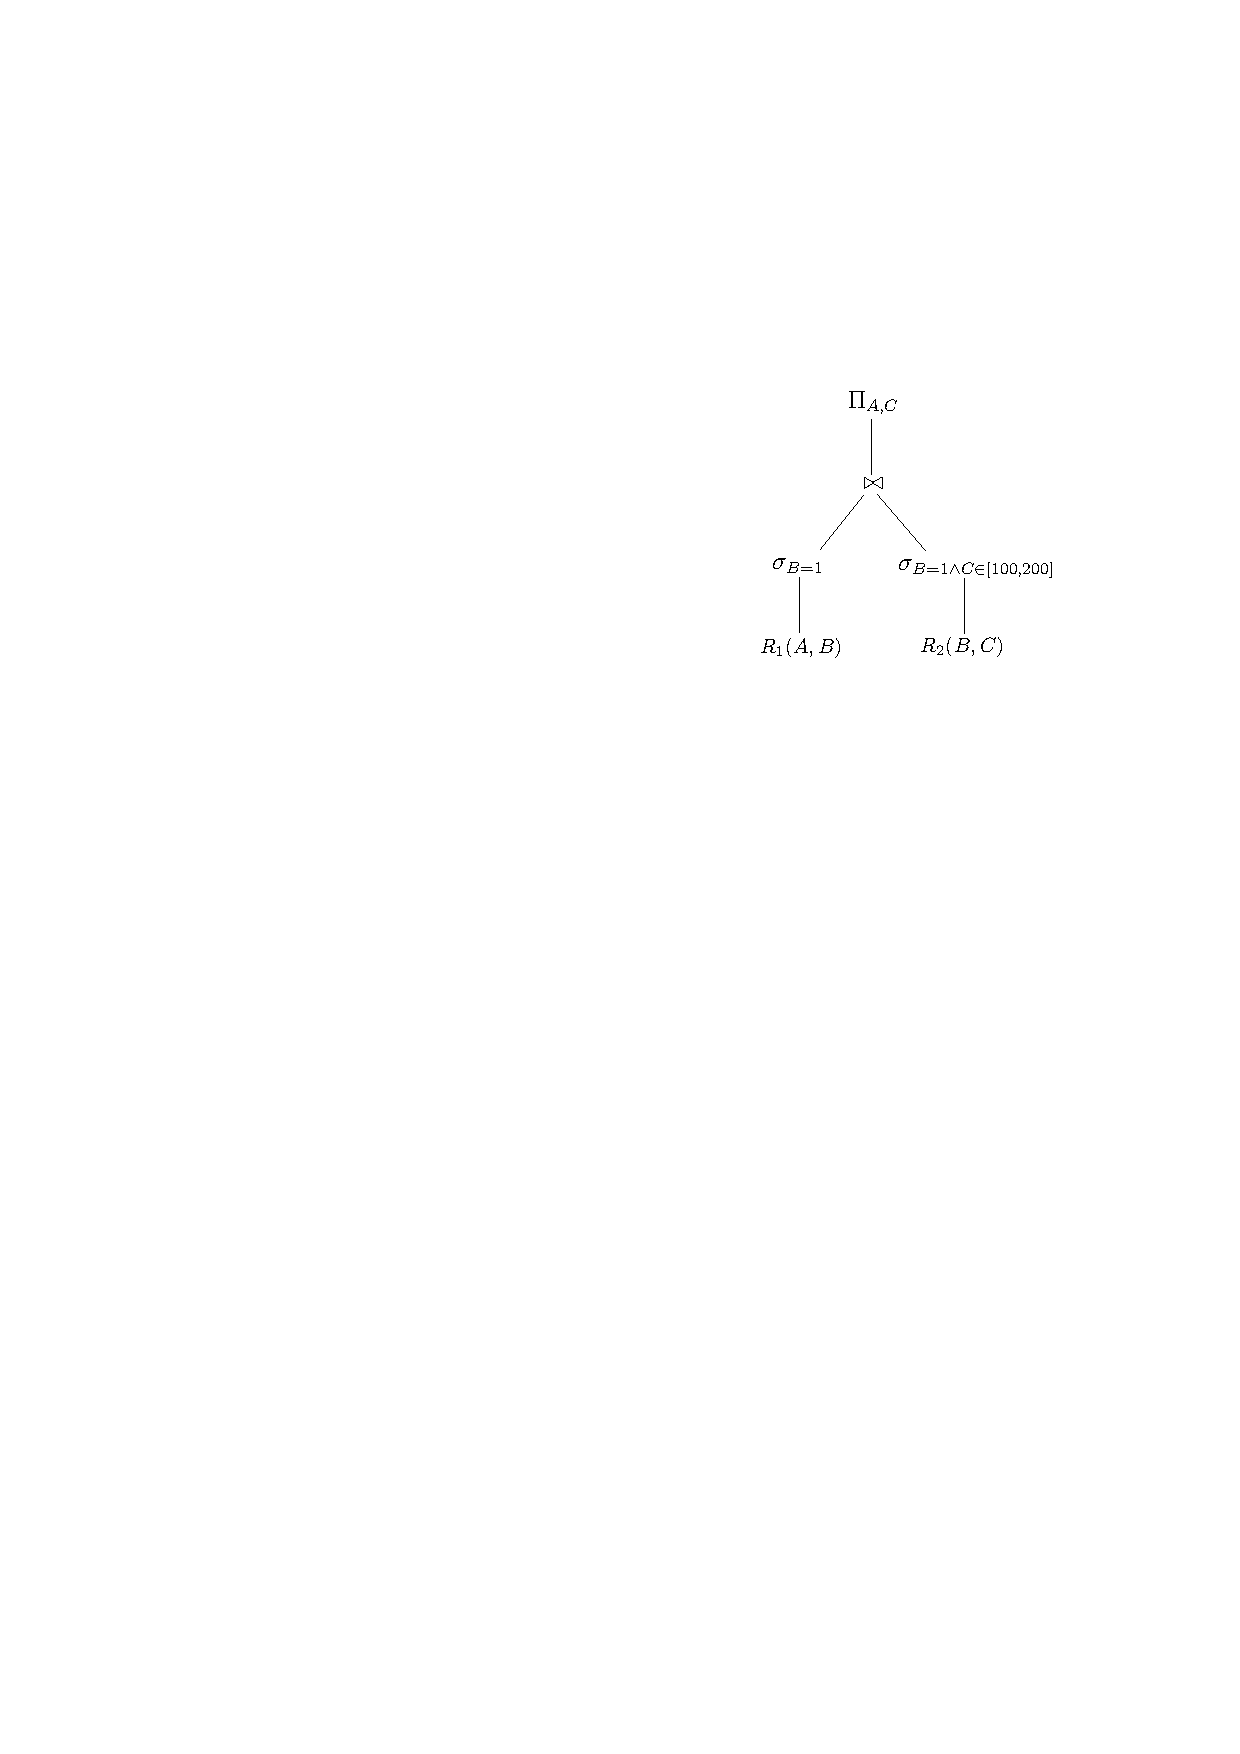
\includegraphics[height=30mm]{./artwork/plan2}
        \end{minipage}
    \end{tabular}

    \vgap

    \mybox[green]{Strategy 5:}
    \begin{itemize}
        \item Compute $\red{R_3} = \sigma_{B=1} R_1$ by reading $R_1$ and materializing $R_3$ \\
        $\Rightarrow$ 10000 (reading) + 1000 (mat.) I/Os \\[-1mm]
        \item Compute $\red{R_4} = \sigma_{B=1 \wedge C \in [100, 200]} R_2$ by reading $R_2$ and materializing $R_4$ $\Rightarrow$ 10000 (reading) + 800 (mat.) I/Os \\[-1mm]
        \item Compute $\red{R_5} = R_3 \bowtie R_4$ with sort join. \\
              \bred{For each tuple $\red{t} \in R_5$ found in memory, output directly $t.A$}. \\
                $\Rightarrow$ $5(1000 + 800)$ I/Os (under no-skew assumption).
    \end{itemize}
    In total: $30800$ I/Os.
}
%-------------------------------------------------------------
\myfrm{
    \cbox{blue}{
        Pipelining may avoid materializing intermediate results altogether.
    }
}
%-------------------------------------------------------------
\myfrm{
    \begin{tabular}{cc}
        %\minipg{0.5\linewidth}{
        \begin{minipage}{0.7\linewidth}
            Assume:
            \myitems{
                \item $\red{B(R_1)} = \red{B(R_2)} = 10000$ \\[-1mm]
                \item $\sigma_{B = 1} R_1 $ has $1000$ blocks. $R_1$ is \bred{clustered} on $B$ and there is a \bred{hash index} on $R_1.B$. \\[-1mm]
                \item $\sigma_{B = 1 \wedge C \in [100, 200]} R_2$ has $800$ blocks  \\[-1mm]
                %\item $\sigma_{B = 1 \wedge C \in [100,200]} R_1 \bowtie R_2$ has $\red{B_2}$ blocks. \\[-1mm]
                \item $\red{M} = 101$.
            }
        \end{minipage}
        &
        \begin{minipage}{0.2\linewidth}
            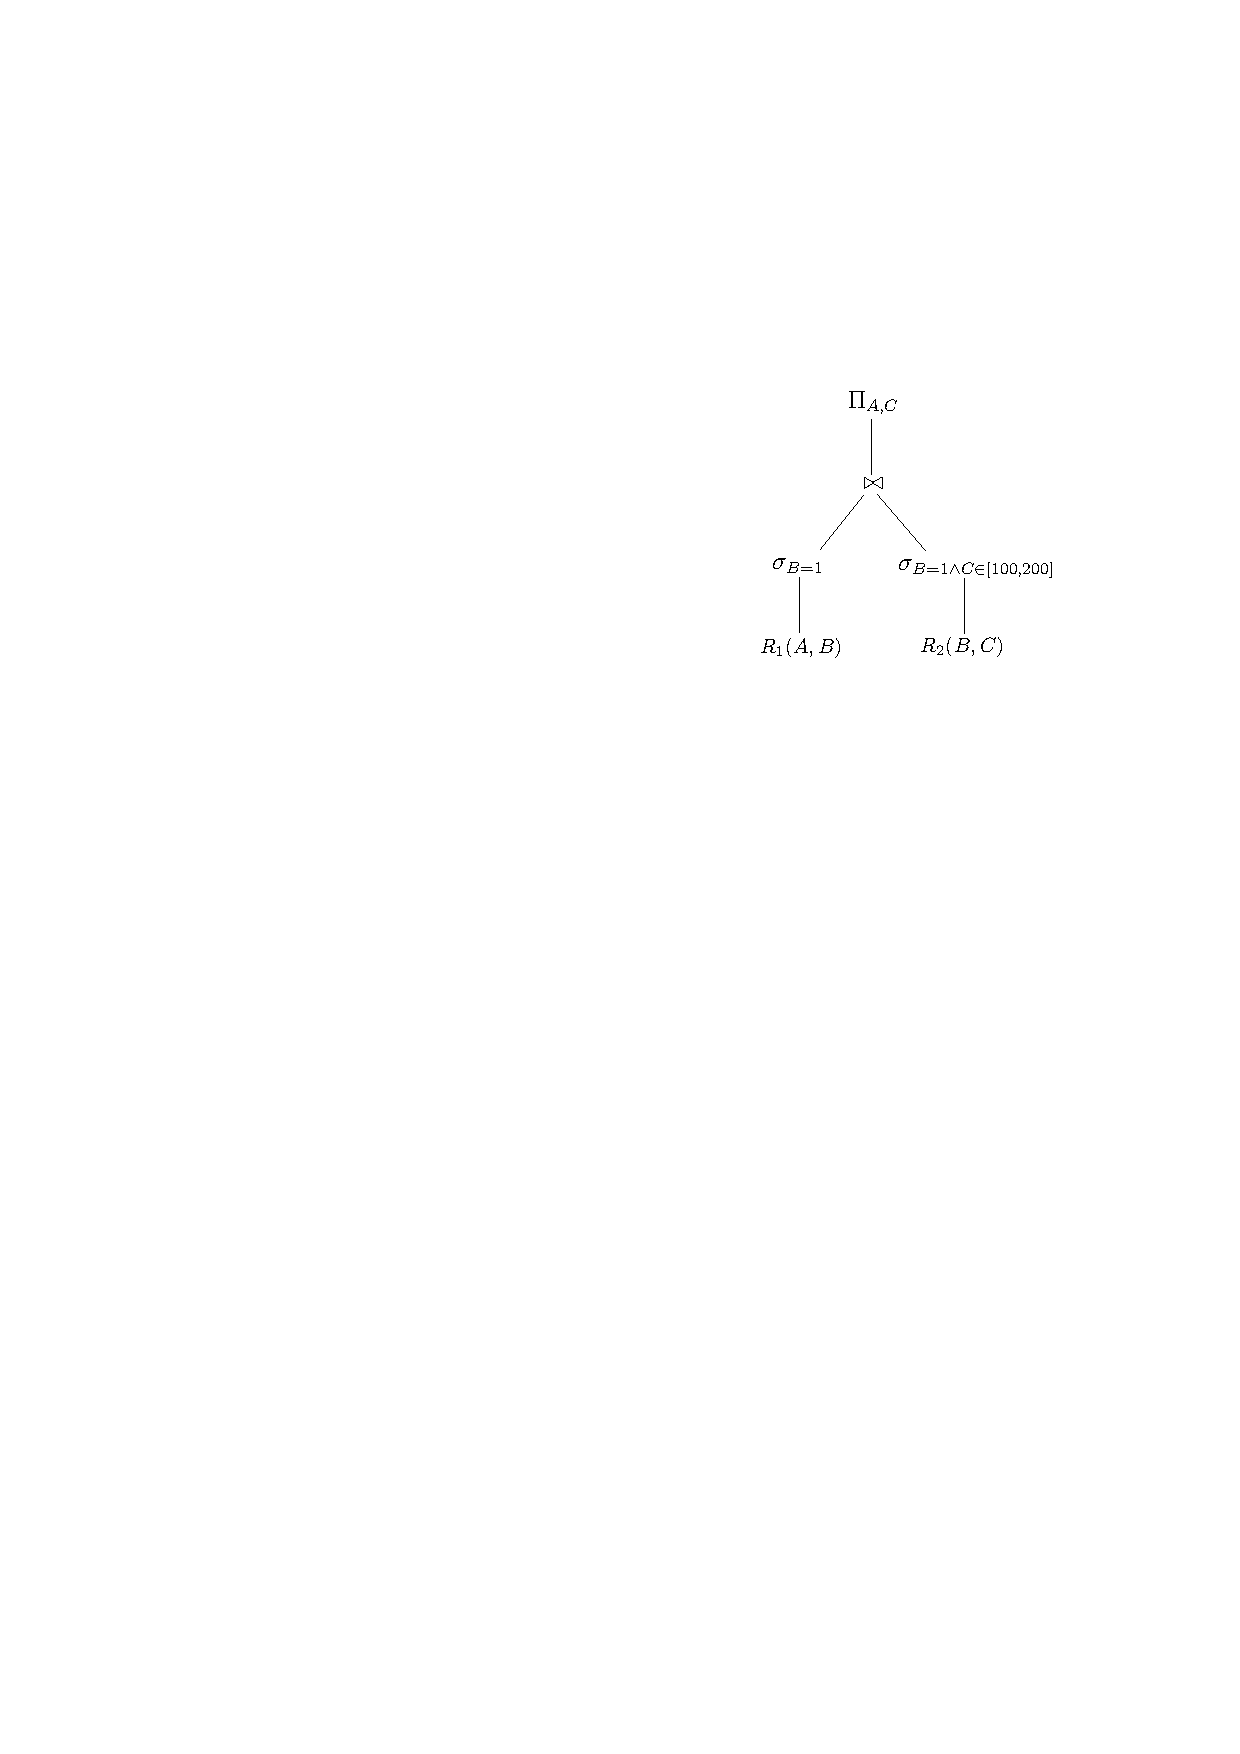
\includegraphics[height=30mm]{./artwork/plan2}
        \end{minipage}
    \end{tabular}

    \vgap

    \mybox[green]{Strategy 6:}
    \begin{itemize}
        \item Compute $\red{R_3} = \sigma_{B=1 \wedge C \in [100, 200]} R_2$ by reading $R_2$ $\Rightarrow$ 10000 I/Os. \\[-1mm]
        \item Using the hash index on $R_1$, we can find $\red{R_4} = \sigma_{B=1} R_1$ in 1 + 1000 = 1001 I/Os. \\[-1mm]
        \item \bred{As soon as getting a tuple} $\red{t} \in R_3$ \bred{in memory}: probe the hash index on $R_1.B$ to find all tuples $\red{s} \in \sigma_{B=1} R_1$; output $(s.A, t.C)$. \\
        $\Rightarrow$ $|R_3| \cdot 1000$ I/Os.
    \end{itemize}
    In total: $10000 + 10000 |R_3|$ I/Os.
}
%-------------------------------------------------------------
\myfrm{
    \begin{tabular}{cc}
        %\minipg{0.5\linewidth}{
        \begin{minipage}{0.7\linewidth}
            Assume:
            \myitems{
                \item $\red{B(R_1)} = \red{B(R_2)} = 10000$ \\[-1mm]
                \item $\sigma_{B = 1} R_1 $ has $1000$ blocks. $R_1$ is \bred{clustered} on $B$ and there is a \bred{hash index} on $R_1.B$. \\[-1mm]
                \item $\sigma_{B = 1 \wedge C \in [100, 200]} R_2$ has $800$ blocks  \\[-1mm]
                %\item $\sigma_{B = 1 \wedge C \in [100,200]} R_1 \bowtie R_2$ has $\red{B_2}$ blocks. \\[-1mm]
                \item $\red{M} = 101$.
            }
        \end{minipage}
        &
        \begin{minipage}{0.2\linewidth}
            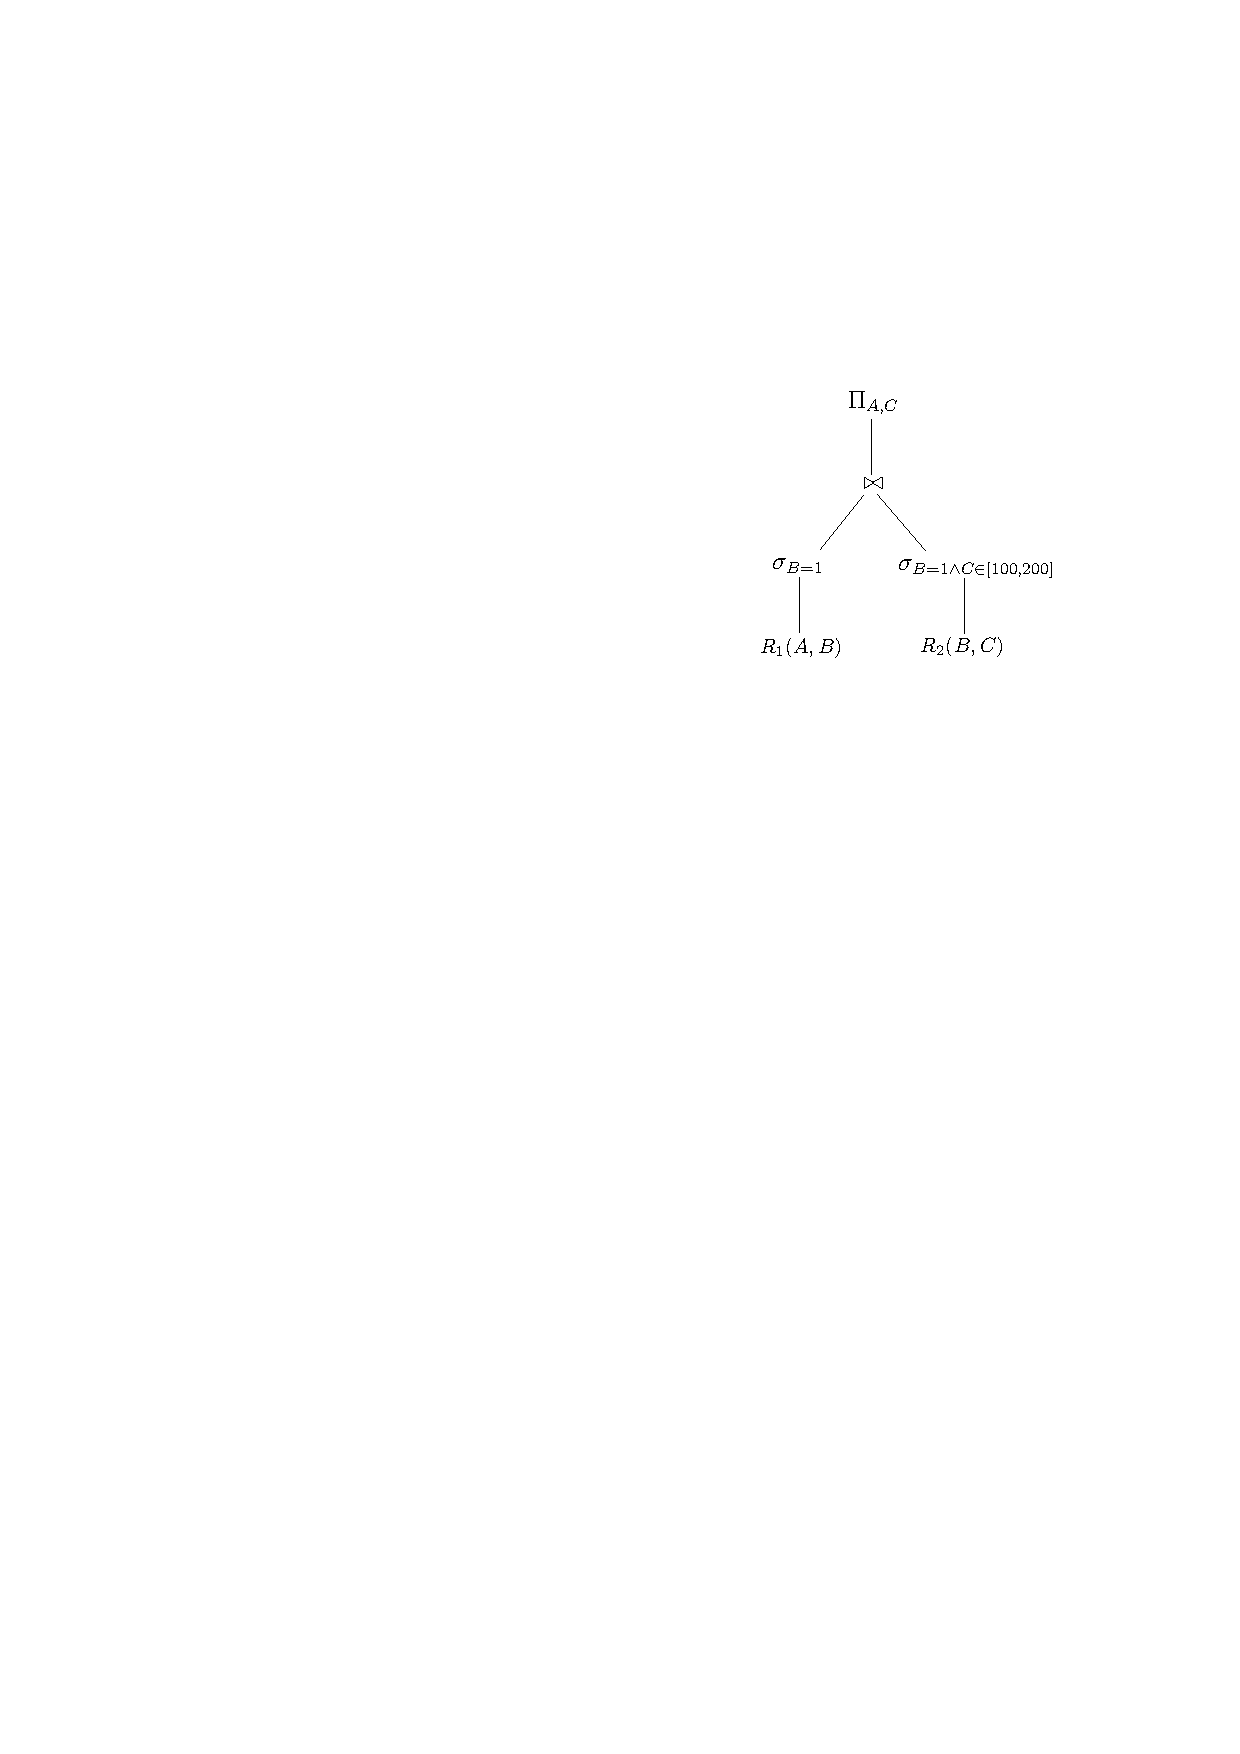
\includegraphics[height=30mm]{./artwork/plan2}
        \end{minipage}
    \end{tabular}

    \vgap

    \mybox[green]{Strategy 7:}
    \begin{itemize}
        \item Compute $\red{R_3} = \sigma_{B=1 \wedge C \in [100, 200]} R_2$ by reading $R_2$ $\Rightarrow$ 10000 I/Os. \\[-1mm]
        \item \bred{Every time we have accumulated $M - 1 = 100$ blocks of new tuples of $R_3$ in memory}, probe the hash index on $R_1.B$ to find $\red{R_4} = \sigma_{B=1} R_1$; output $(s.A, t.C)$ for each $\red{t} \in R_3$ in memory and every $\red{s} \in R_4$ \\
        $\Rightarrow$ $\lc 800/100 \rc \cdot 1001 = 8008$ I/Os.
    \end{itemize}
    In total: $18008$ I/Os.
}
%-------------------------------------------------------------
\myfrm{
    \cbox{green}{
        Query optimization is an art. It is an active research area.

        \vgap

        The methods we discussed are representative but far from being comprehensive. The query optimization module of a database system is a highly sophisticated and often kept as a commercial secret.
    }
}
%-------------------------------------------------------------
\end{document} 


